% -----------------------------------------------------------------------------
\section{Conventions}
% -----------------------------------------------------------------------------

This section provides some preliminary information to aid in the understanding of the specification.
The SBOL data model is specified using Unified Modeling Language (UML) 2.0 diagrams \href{http://www.omg.org/spec/UML/2.0/}{(OMG 2005)}. This section reviews terminology conventions, the basics of UML diagrams, and our naming conventions.

\subsection{Terminology Conventions}

This document indicates requirement levels using the controlled vocabulary specified in \href{https://tools.ietf.org/html/rfc2119}{IETF RFC 2119}.
In particular, the key words ``MUST'', ``MUST NOT'', ``REQUIRED'', ``SHALL'', ``SHALL NOT'', ``SHOULD'', ``SHOULD NOT'', ``RECOMMENDED'', ``MAY'', and ``OPTIONAL'' in this document are to be interpreted as described in RFC 2119.

\begin{itemize}
\item The words ``MUST'', ``REQUIRED'', or ``SHALL'' mean that the item is an absolute requirement.
\item The phrases ``MUST NOT'' or ``SHALL NOT'' mean that the item is an absolute prohibition.
\item The word ``SHOULD'' or the adjective ``RECOMMENDED'' mean that there might exist valid reasons in particular circumstances to ignore a particular item, but the full implications need to be understood and carefully weighed before choosing a different course.
\item The phrases ``SHOULD NOT'' or ``NOT RECOMMENDED'' mean that there might exist valid reasons in particular circumstances when the particular behavior is acceptable or even useful, but the full implications needs to be understood and the case carefully weighed before implementing any behavior described with this label.
\item The word ``MAY'' or the adjective ``OPTIONAL'' mean that an item is truly optional.
\end{itemize}

\subsection{UML Diagram Conventions}
\label{sec:umldiagrams}

The types of data modeled by OPIL are commonly referred to as {\em classes}, especially when discussing the details of software implementation. Each OPIL class can be instantiated by many OPIL objects. These objects MAY contain data that differ in content, but they MUST agree on the type and form of their data as dictated by their common class. Classes are represented in UML diagrams as rectangles labeled at the top with class names (see \ref{fig:uml_sampler} for examples).

\begin{figure}[ht]
\begin{center}
  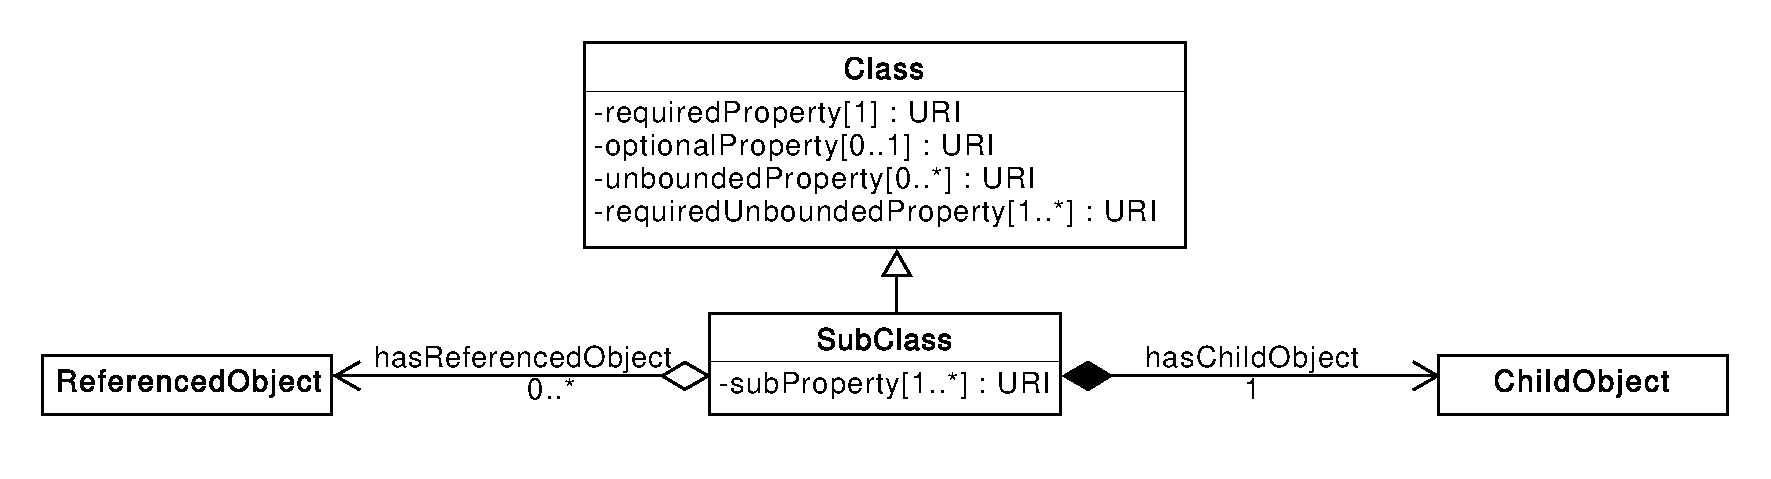
\includegraphics[width=\textwidth]{figures/uml_sampler.pdf}
\caption{Examples of UML diagram conventions used in this document}
\label{fig:uml_sampler}
\end{center}
\end{figure}

Classes can be connected to other classes by association properties, which are represented in UML diagrams as arrows. These arrows are labeled with data cardinalities in order to indicate how many values a given association property can possess (see below). The remaining (non-association) properties of a class are listed below its name. Each of the latter properties is labeled with its data type and cardinality.

In the case of an association property, the class from which the arrow originates is the owner of the association property. A diamond at the origin of the arrow indicates the type of association.
Open-faced diamonds indicate shared aggregation, also known as a reference, in which the owner of the association property exists independently of its value.

By contrast, filled diamonds indicate composite aggregation, also known as a part-whole relationship, in which the value of the association property MUST NOT exist independently of its owner.
In addition, in the OPIL data model, it is REQUIRED that the value of each composite aggregation property is a unique OPIL object (that is, not the value for more than one such property).
Note that in all cases, composite aggregation is used in such a way that there SHOULD NOT be duplication of such objects.
Such objects are also commonly referred to as ``child'' objects, and their owning objects as ``parent'' objects.

All OPIL properties are labeled with one of several restrictions on data cardinality. These are:

\begin{itemize}

\item $1$ - REQUIRED: there MUST be exactly one value for this property.

\item $0 \ldots 1$ - OPTIONAL: there MAY be a single value for this property, or it MAY be absent.

\item $0 \ldots *$ - zero or more: there MAY be any number of values for this property, including none.

\item $1 \ldots *$ - REQUIRED, one or more: there MAY be any number of values for this property, as long as there is at least one.

\item $n \ldots *$ - at least: there MUST be at least $n$ values for this property.

\end{itemize}

Finally, classes can inherit the properties of other classes. Inheritance relationships are represented in UML diagrams as open-faced, triangular arrows that point from the inheriting class to the inherited class. Some classes in the OPIL data model cannot be instantiated as objects and exist only to group common properties for inheritance. These classes have italicized names and are known as abstract classes.

\subsection{Naming and Typographic Conventions}
\label{sec:nameconventions}

OPIL classes are named using upper ``camel case,'' meaning that each word is capitalized and all words are run together without spaces, e.g., \opil{ProtocolInterface}.
Properties, on the other hand, are named using lower camel case, meaning that they begin lowercase but if they consist of multiple words, all words after the first begin with an uppercase letter (e.g., \opil{hasParameter}).

OPIL properties are always given singular names irrespective of their cardinality, e.g., \opil{hasParameter} is used rather than \opil{hasParameters} even though a \opil{ProtocolInterface} can have multiple parameters.
This is because each relation can potentially stand on its own, irrespective of the existence of others in the set.

Two conventions are used for property names, {\tt name} and {\tt hasName}.  
When a property is pointing to a class using the same name, it uses the {\tt hasName} convention (e.g., the \opil{ProtocolInterface} class uses \opil{hasParameter} to point to a \opil{Parameter} object).
When the property uses a different name than the class of the object it points to, it uses the {\tt name} convention instead (e.g., the \opil{MeasurementType} class uses \opil{minInterval} to point to a \opil{Measure} object).



